\chapterimage{recursos.jpg} % Table of contents heading image
\chapter{Recursos Físicos}
\section{Diagrama de Nodos/Emplazamiento}

Los diagramas de nodos o emplezamiento se encargan de representar los recursos físicos usados por el programa y sus componentes, es decir, que si el programa se divide en, por ejemplo, cliente-servidor, este diagrama muestra los recursos principales de los mismos. Esto permite dimencionar en parte el costo computacional que requiere el programa, y las características de las máquinas en donde puede ser usado. En caso de que el programa no requiere nada superlativo para su montage, el diagrama solo mostrara el uso de los recursos basico que son CPU y RAM.

\begin{figure}[H]
	\centering
	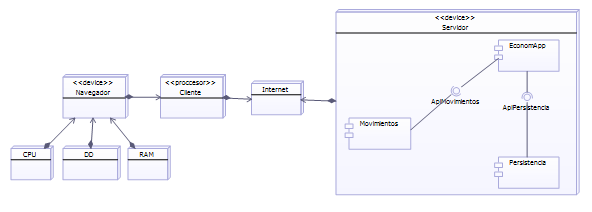
\includegraphics[width=1\linewidth]{parte2/imgs/DiagramaDeNodos/Nodos}
	\caption{Diagrama de Nodos}
	\label{fig:nodos}
\end{figure}

Como el programa es la interacción de un cliente y un servidor, entonces el servidor es el que carga con praticamente todo el procesamiento propio de la aplicacion, mientras que el cliente actua como ventana de para el usuario final, que consumira el api del mismo a travez de internet. Ya que el cliente está inicialmente usando una aplicacion web, el recurso del sistema en ese momento es el navegador, el cual nos provee el consumo de ram, disco duro y procesador, independiente de la aplicación.
